\documentclass[a4paper,12pt]{book}
\usepackage[utf8]{inputenc}
\usepackage{graphicx}
\usepackage{hyperref}
\usepackage{makecell}
\usepackage{array}
\newcolumntype{L}[1]{>{\raggedright\let\newline\\\arraybackslash\hspace{0pt}}m{#1}}
\newcolumntype{C}[1]{>{\centering\let\newline\\\arraybackslash\hspace{0pt}}m{#1}}
\newcolumntype{R}[1]{>{\raggedleft\let\newline\\\arraybackslash\hspace{0pt}}m{#1}}
\begin{document}

\author{TeXstudio Team}
\title{Simple Book Example}
\date{January 2013}

\frontmatter
\maketitle
\tableofcontents

\mainmatter
\chapter{The First Chapter}
\chapter{Regression}
\section{Evaluating Regression Models Performance}
R square
\begin{equation}
SS_{hot}=SUM(y_i-y_{avg})^2
\end{equation}
\begin{equation}
SS_{hot}=SUM(y_i-y_{avg})^2
\end{equation}
\begin{equation}
R^2=1-\frac{SS_{res}}{SS_{tot}}
\end{equation}
Here, we want $SS_{res} \rightarrow Min$

The problem here is: if we have $n$ features (regressor) have been already existed in our regression model. We will add a new feature, we want to know if it helps to improve the performance of hour model. The solution is: we compare the difference of $R^2$ with and without the new feature. There are two situations here:
\begin{enumerate}
	\item $R^2$ increase. Because the new feature decrease the $SS_{res}$
	\item $R^2$ keeps unchanged. Because the new feature does not help the model. It has no effect on the dependant variable. The coefficient of the new feature is zero.
\end{enumerate}
When add a new feature, it is bias as the $R^2$ is always increase. So the adjust $R$ square is proposed.
\begin{equation}
Adj R^2 = 1- (1 - R^2)\frac{n-1}{n-p-1},
\end{equation}
where $p$ is the number of regressors and $n$ is the sample size.

One example is shown as follows:
\begin{figure}
	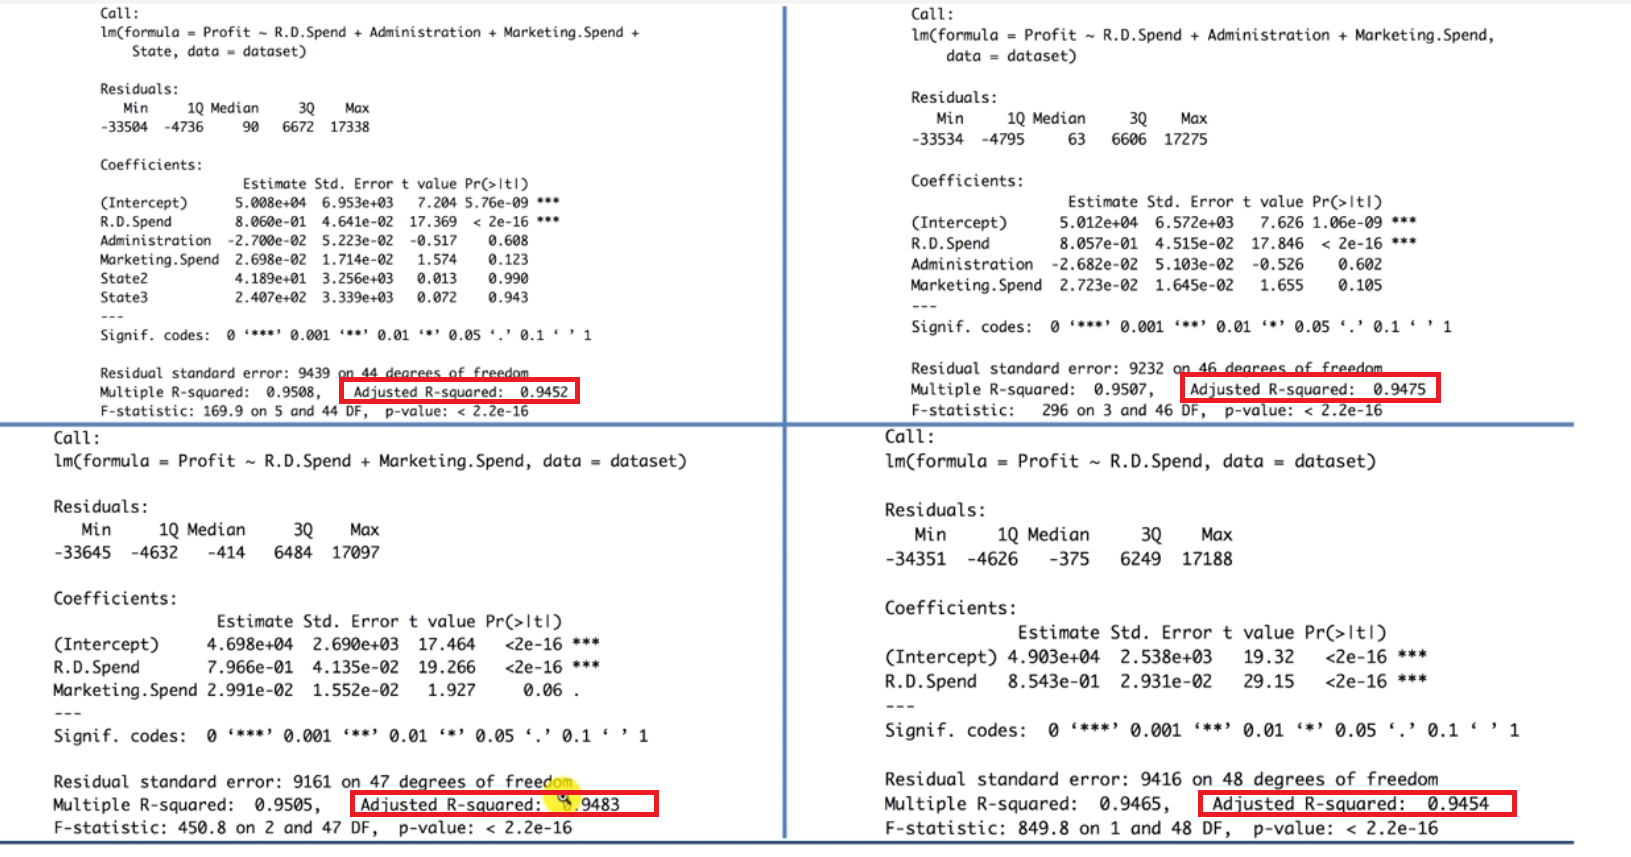
\includegraphics[width=\linewidth]{./figures/adjust_r_square.png}
	\centering
	\caption{example of adjust square error}
\end{figure}

\begin{table}
	\begin{tabular}{ | C{0.33\linewidth} | C{0.33\linewidth}| C{0.33\linewidth} | } 
		\hline
		Regression Model & Pros & Cons \\ 
		\hline
		Linear Regression &  Works on any size of dataset, gives information about relevance of features & The Linear Regression Assumptions \\
		\hline 
		Polynomial Regression & works on any size of dataset, works very well on non linear problems & Need to choose the right polynomial degree for a good bias/variance tradeoff \\ 
		\hline
		SVR & Easily adaptable, works very well on non linear problems, not biased by outliers & Compulsory to apply feature scaling, not well known, more difficult to understand \\
		\hline
		Decision Tree Regression & Interpretability, no need for feature scaling, works on both  linear/nonlinear problems & Poor results on too small datasets, overfitting can easily occur\\
		\hline
		Random Forest Regression & powerful and accurate, good performance on many problems, including non linear & Nointerpretability, overfitting can easily occur, need to choose the number of trees\\
		\hline
	\end{tabular}
\caption{Comparison of different regression models}
\label{table:comp}
\end{table}
Table \ref{table:comp} shows the comparison of different regression models from  \href{https://www.superdatascience.com/wp-content/uploads/2017/02/Regression-Pros-Cons.pdf}{comparison}.

How to address overfitting problems:\href{https://www.superdatascience.com/wp-content/uploads/2017/02/Regularization.pdf}{Regularization}.

\chapter{Classification}

\section{Logistic Regression}
Logistic regression is a linear regression, which returns the possibility.
\begin{equation}
y = b_0 + b_1*x
\end{equation}
\begin{equation}
p = \frac{1}{1+e^{-y}}
\end{equation}

How to evaluate the performance of classification:
$confusion\_{matrix}(y_{true}, y_{pred})$

By definition a confusion matrix $C$ is such that $C_{i, j}$ is equal to the number of observations known to be in group $i$ but predicted to be in group $j$.
Thus in binary classification, the count of true negatives is $C_{0,0}$, false negatives is $C_{1,0}$, true positives is $C_{1,1}$ and false positives is $C_{0,1}$

How to understand true positive, false positive, true negative, false negative, recall, precision?

Suppose a computer program for recognizing dogs in photographs identifies eight dogs in a picture containing 12 dogs and some cats. Of the eight dogs identified, five actually are dogs (true positives), while the rest are cats (false positives). The program's precision is 5/8 while its recall is 5/12. When a search engine returns 30 pages only 20 of which were relevant while failing to return 40 additional relevant pages, its precision is 20/30 = 2/3 while its recall is 20/60 = 1/3. So, in this case, precision is ``how useful the search results are'', and recall is ``how complete the results are''.

\begin{figure}
	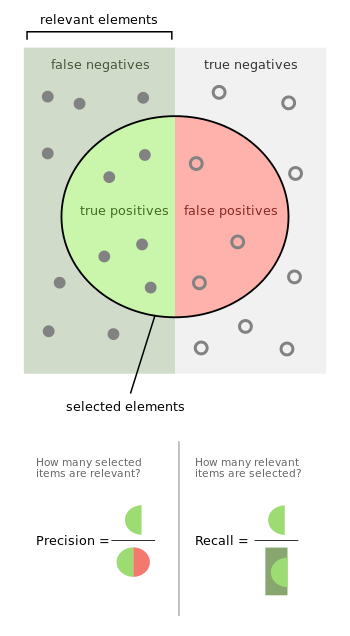
\includegraphics[width=\linewidth]{./figures/precision_recall.png}
	\centering
	\caption{example of precision and recall}
\end{figure}

\section{K-Nearest Neighbors (K-NN)}
\begin{enumerate}
	\item choose the number $K$ of neighbours
	\item take the $K$ nearest neighbours of the new data point, according to the Euclidean distance
	\item among these $K$ neighbours, count the number of data points in each category
	\item assign the new data point to the category where you counted the most neighbours
\end{enumerate}
\section{Support Vector Machine (SVM)}

\section{Kernel SVM}

\section{Naive Bayes}

\section{Decision Tree Classification}

\section{Random Forest Classification}

\section{Evaluating Classification Models Performance}
\chapter{Clustering}
\section{K-Means Clustering}
\section{Hierarchical Clustering}


\backmatter
% bibliography, glossary and index would go here.

\end{document}